\documentclass[11pt,a4paper]{article}

% Encodage
\usepackage[utf8]{inputenc}
\usepackage[T1]{fontenc}
\usepackage[french]{babel}

% Mise en page
\usepackage{geometry}
\geometry{margin=2.5cm}
\usepackage{setspace}
\onehalfspacing

% Liens & hypertextes
\usepackage{hyperref}

% Maths & figures
\usepackage{amsmath,amssymb}
\usepackage{graphicx}
\usepackage{float} % Pour forcer la position des figures
\usepackage{caption}

% Couleurs (facultatif)
\usepackage{xcolor}

% Infos du document
\title{\textbf{Compte Rendu de Projet -- Génération d'image par Algorithmes Génétiques}}
\author{Marianne B. -- Double Majeure Informatique}
\date{\today}


\begin{document}

\maketitle

\section{Introduction}
Ce projet a pour objectif de générer automatiquement une image imitant une image cible à l'aide d'algorithmes génétiques. L'image est reconstituée par un assemblage de traits de pinceau simulés (brush strokes), selon une logique d'évolution inspirée de la biologie.

\section{Contexte et Objectifs}
L'idée est de commencer avec une population d'images générées aléatoirement, chacune composée de formes primitives (triangles, ellipses, traits, etc.). Ces formes évoluent au fil des générations pour ressembler de plus en plus à une image cible. Cela nous permet d'appliquer des concepts de sélection, mutation, croisement et évaluation de fitness à un problème visuel.

\section{Conception Algorithmique}
\subsection{Représentation des individus}
Chaque image est représentée comme un ensemble de "brushs" décrits par :
\begin{itemize}
    \item Position $(x, y)$
    \item Taille et rotation
    \item Couleur $(r, g, b)$ et opacité
    \item ID de brush utilisé dans la bibliothèque
\end{itemize}

\subsection{Évolution}
Nous utilisons une boucle d'évolution avec :
\begin{itemize}
    \item Sélection des meilleurs individus (selNSGA2)
    \item Croisement (crossover uniforme)
    \item Mutation (paramètres légèrement modifiés)
    \item Fitness calculée par distance perceptuelle (LAB + deltaE)
    \item Recherche de nouveauté (HOG + distance entre individus)
\end{itemize}

\subsection{Améliorations guidées}
\begin{itemize}
    \item K-means sur les bords pour mieux positionner les brushs
    \item Gradient de Sobel pour guider la direction des traits
    \item Évolution par phases (coarse-to-fine)
\end{itemize}

\section{Implémentation Technique}
Le projet est structuré autour de trois modules Python :
\begin{itemize}
    \item \texttt{core/brush.py} : classe \texttt{BrushStroke}, encodage génétique
    \item \texttt{core/painting.py} : rendu de l'image, détection de bords, génération de GIF
    \item \texttt{core/solver.py} : algorithme d'évolution avec DEAP
\end{itemize}

Un notebook Jupyter permet d'exécuter les tests et d'afficher les résultats facilement.

\section{Expérimentations}
Nous avons testé le système sur plusieurs images (Mario, arbre, etc.). Voici un exemple de résultat après 100 générations :

\begin{figure}[H]
    \centering
    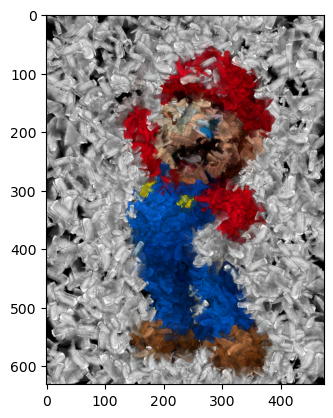
\includegraphics[width=0.6\textwidth]{images/mario_result.png}
    \caption{Image générée à partir de Mario après 100 générations}
\end{figure}

Nous avons constaté que :
\begin{itemize}
    \item L'algorithme converge rapidement sur les images simples
    \item Le gradient améliore l'alignement des traits
    \item La recherche de nouveauté évite la stagnation
\end{itemize}

\section{Conclusion}
Ce projet nous a permis d'appliquer des techniques avancées d'optimisation évolutionnaire à un problème visuel original. Le code reste modulaire et pourrait être amélioré par :
\begin{itemize}
    \item L'ajout de textures
    \item L'intégration de réseaux de neurones
    \item L'utilisation de masques manuels
\end{itemize}

\vfill
\noindent\textbf{Date de rendu du rapport :} 26 juin 2025 à 23h59 \\
\textbf{Durée de la soutenance :} 20 minutes de présentation, 5 minutes de questions

\end{document}
